% Requires: \usepackage{graphicx,tikz}
% Image paths are relative to this .tex file's location.
% Generated by: smixae latex figures  (experiment: gemma_2_9b_l11)

\begin{figure*}[t]
\centering
\noindent\makebox[\linewidth][c]{%
\begin{minipage}[t]{\linewidth}%
\vspace{0pt}\centering%
\begin{minipage}[c][4.0cm][c]{0.3267\linewidth}%
\centering%
\begin{tikzpicture}[baseline=(img.base)]
  \node[inner sep=0pt] (img) {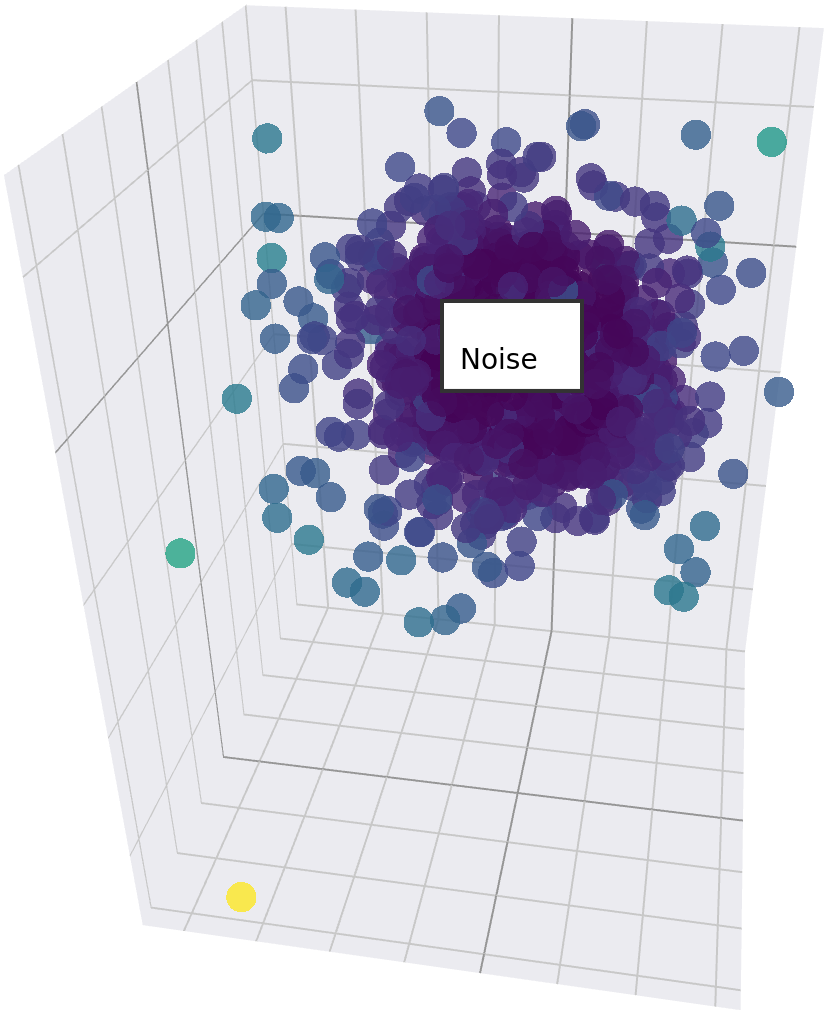
\includegraphics[width=\linewidth,height=4.0cm,keepaspectratio]{paper/camera_ready/gemma_2_9b_l11__continuity__E1326__random__cont__0.3779__scatter.png}};
  \node[anchor=north west, inner sep=2pt, overlay] at (img.north west) {\small\textbf{(a)}};
\end{tikzpicture}%
\end{minipage}%
\begin{minipage}[c][4.0cm][c]{0.3267\linewidth}%
\centering%
\begin{tikzpicture}[baseline=(img.base)]
  \node[inner sep=0pt] (img) {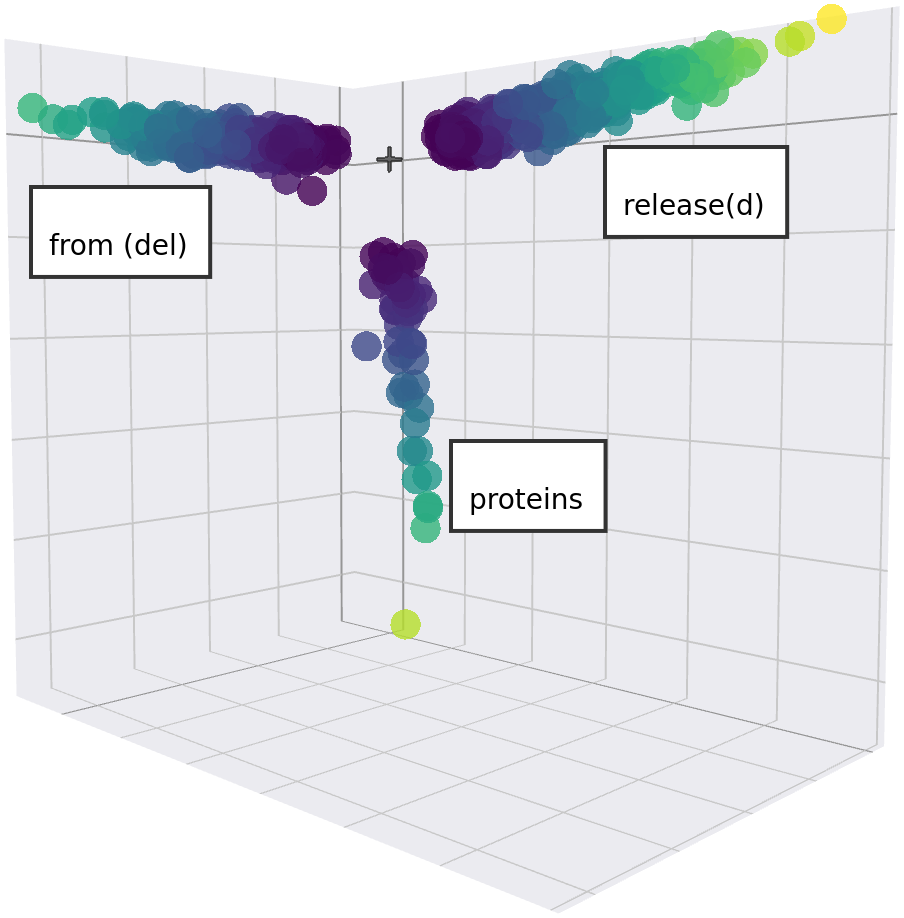
\includegraphics[width=\linewidth,height=4.0cm,keepaspectratio]{paper/camera_ready/gemma_2_9b_l11__continuity__E1527__random__cont__0.5184__scatter.png}};
  \node[anchor=north west, inner sep=2pt, overlay] at (img.north west) {\small\textbf{(b)}};
\end{tikzpicture}%
\end{minipage}%
\begin{minipage}[c][4.0cm][c]{0.3267\linewidth}%
\centering%
\begin{tikzpicture}[baseline=(img.base)]
  \node[inner sep=0pt] (img) {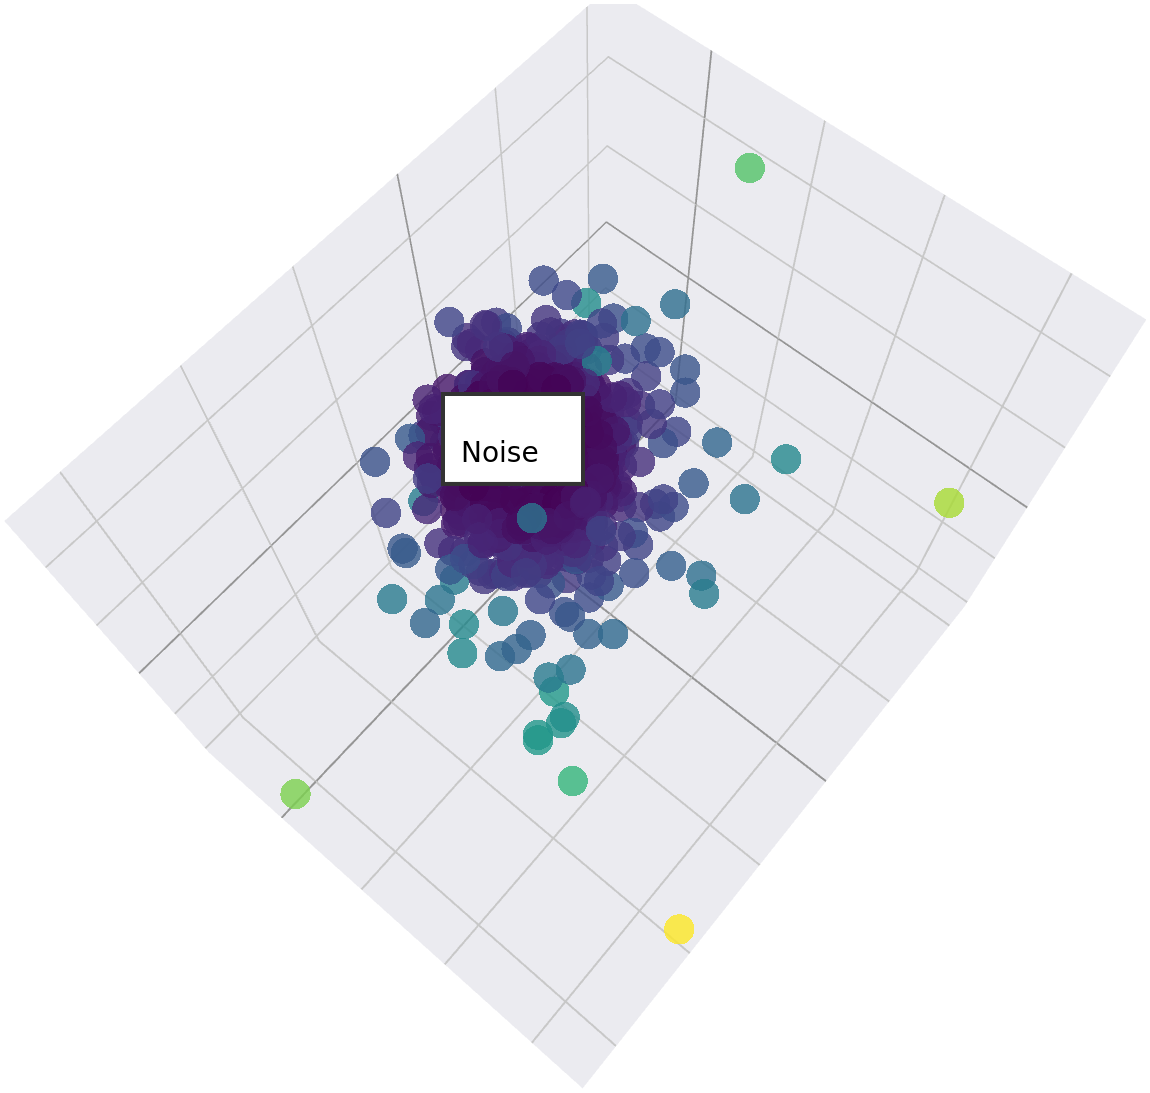
\includegraphics[width=\linewidth,height=4.0cm,keepaspectratio]{paper/camera_ready/gemma_2_9b_l11__continuity__E1537__random__cont__0.3663__scatter.png}};
  \node[anchor=north west, inner sep=2pt, overlay] at (img.north west) {\small\textbf{(c)}};
\end{tikzpicture}%
\end{minipage}%
\par\vspace{3pt}%
\begin{minipage}[c][4.0cm][c]{0.3267\linewidth}%
\centering%
\begin{tikzpicture}[baseline=(img.base)]
  \node[inner sep=0pt] (img) {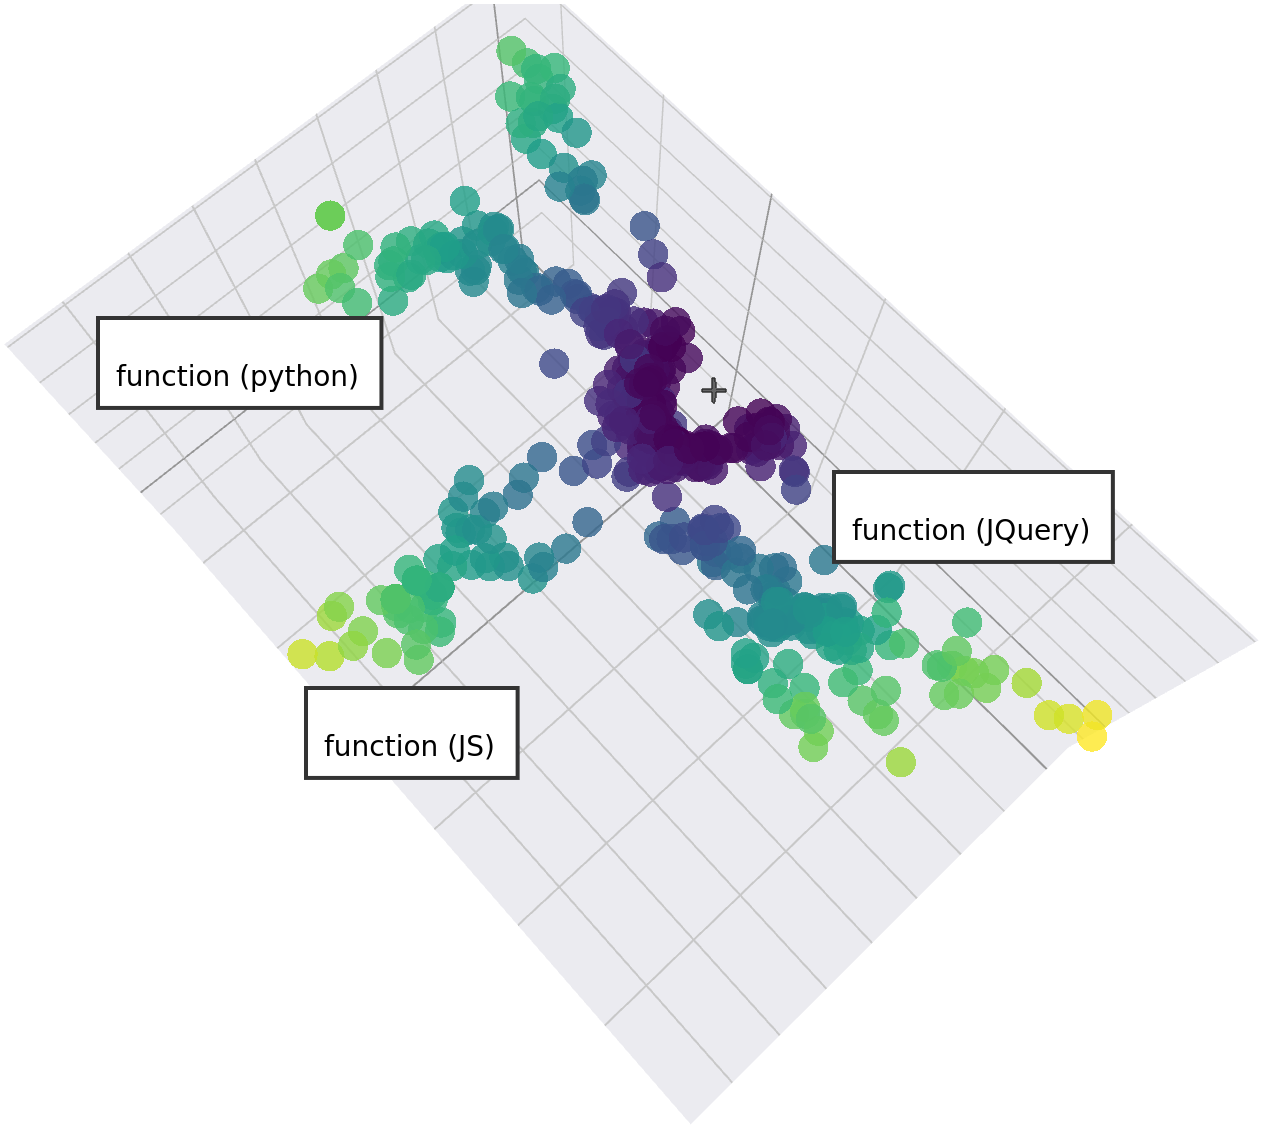
\includegraphics[width=\linewidth,height=4.0cm,keepaspectratio]{paper/camera_ready/gemma_2_9b_l11__continuity__E210__random__cont__0.6363__scatter.png}};
  \node[anchor=north west, inner sep=2pt, overlay] at (img.north west) {\small\textbf{(d)}};
\end{tikzpicture}%
\end{minipage}%
\begin{minipage}[c][4.0cm][c]{0.3267\linewidth}%
\centering%
\begin{tikzpicture}[baseline=(img.base)]
  \node[inner sep=0pt] (img) {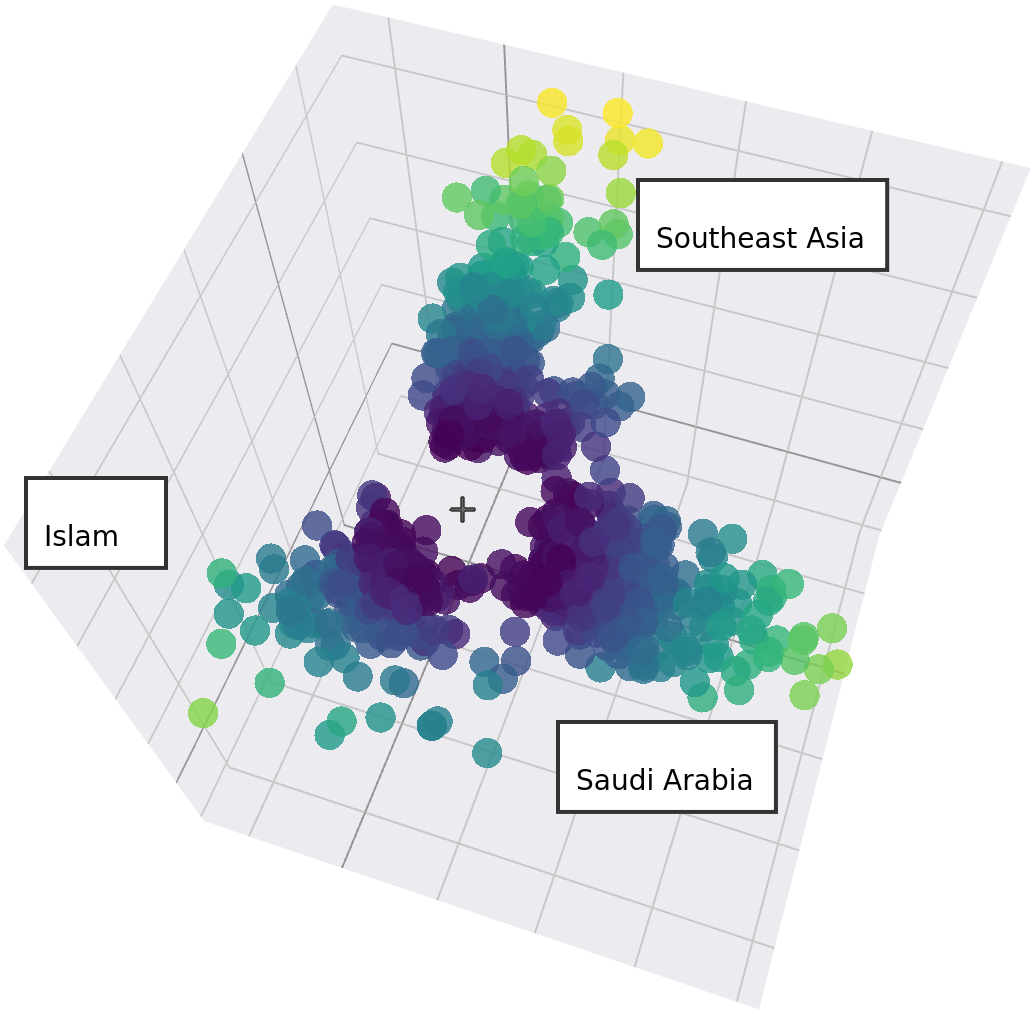
\includegraphics[width=\linewidth,height=4.0cm,keepaspectratio]{paper/camera_ready/gemma_2_9b_l11__continuity__E229__random__cont__0.4197__scatter.png}};
  \node[anchor=north west, inner sep=2pt, overlay] at (img.north west) {\small\textbf{(e)}};
\end{tikzpicture}%
\end{minipage}%
\begin{minipage}[c][4.0cm][c]{0.3267\linewidth}%
\centering%
\begin{tikzpicture}[baseline=(img.base)]
  \node[inner sep=0pt] (img) {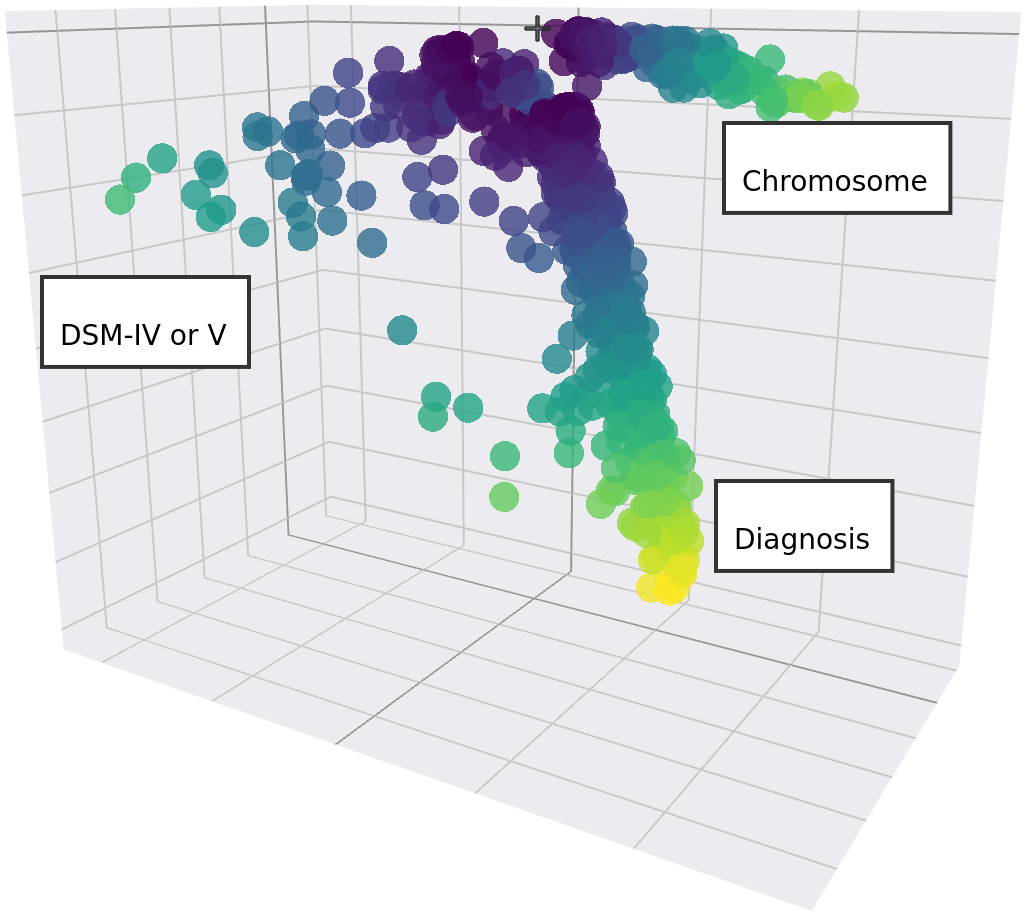
\includegraphics[width=\linewidth,height=4.0cm,keepaspectratio]{paper/camera_ready/gemma_2_9b_l11__continuity__E289__random__cont__0.5605__scatter.png}};
  \node[anchor=north west, inner sep=2pt, overlay] at (img.north west) {\small\textbf{(f)}};
\end{tikzpicture}%
\end{minipage}%
\par\vspace{3pt}%
\begin{minipage}[c][4.0cm][c]{0.3267\linewidth}%
\centering%
\begin{tikzpicture}[baseline=(img.base)]
  \node[inner sep=0pt] (img) {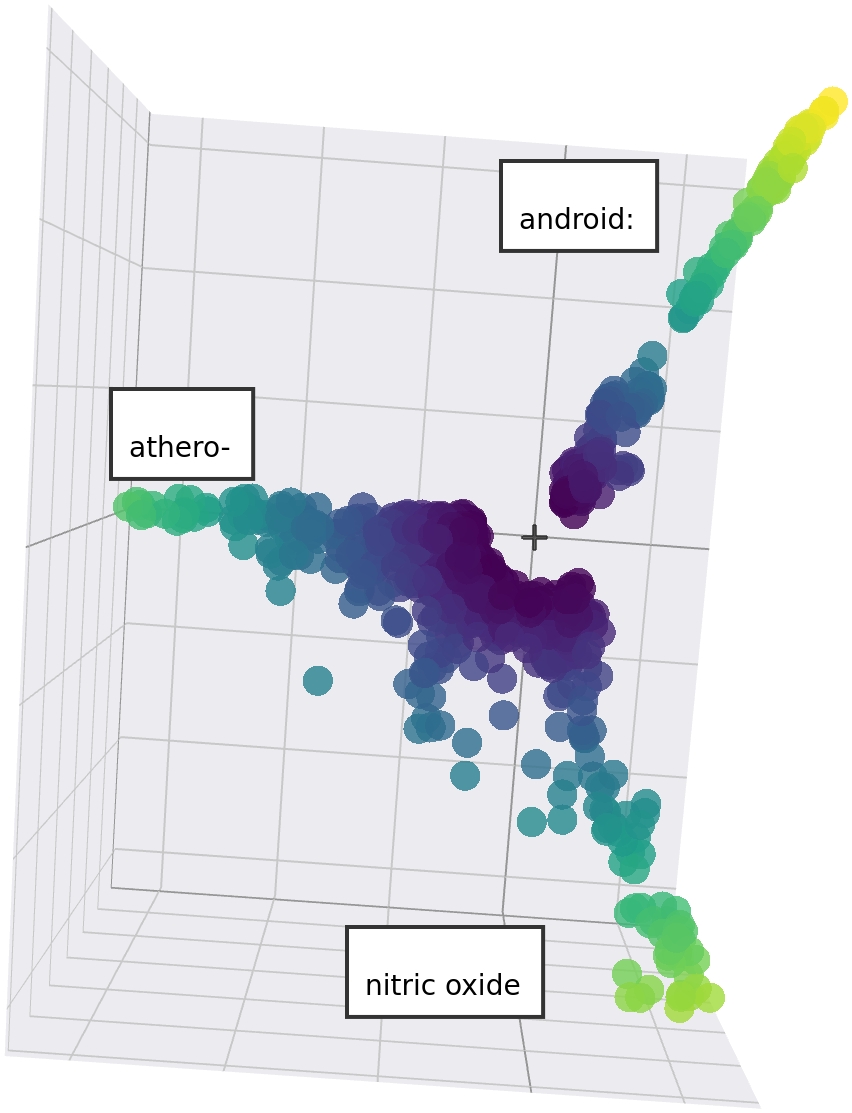
\includegraphics[width=\linewidth,height=4.0cm,keepaspectratio]{paper/camera_ready/gemma_2_9b_l11__continuity__E464__random__cont__0.5773__scatter.png}};
  \node[anchor=north west, inner sep=2pt, overlay] at (img.north west) {\small\textbf{(g)}};
\end{tikzpicture}%
\end{minipage}%
\begin{minipage}[c][4.0cm][c]{0.3267\linewidth}%
\centering%
\begin{tikzpicture}[baseline=(img.base)]
  \node[inner sep=0pt] (img) {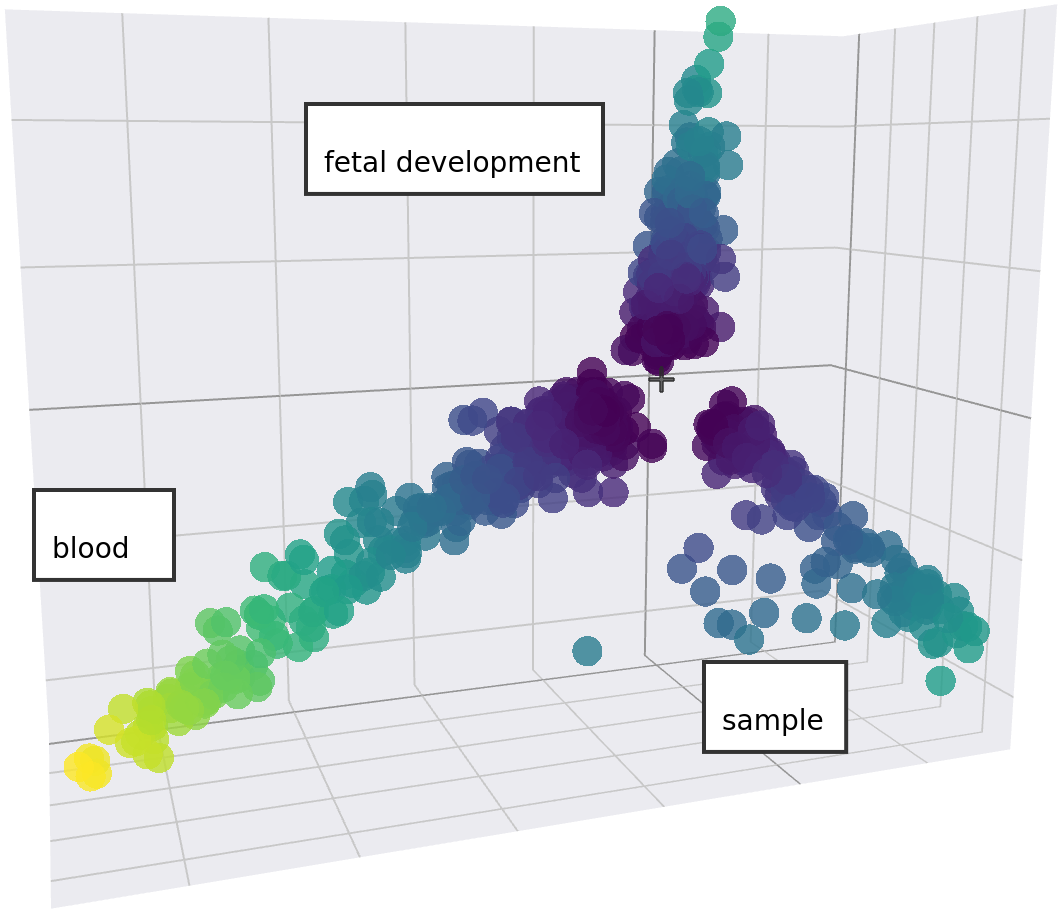
\includegraphics[width=\linewidth,height=4.0cm,keepaspectratio]{paper/camera_ready/gemma_2_9b_l11__continuity__E508__random__cont__0.5031__scatter.png}};
  \node[anchor=north west, inner sep=2pt, overlay] at (img.north west) {\small\textbf{(h)}};
\end{tikzpicture}%
\end{minipage}%
\begin{minipage}[c][4.0cm][c]{0.3267\linewidth}%
\centering%
\begin{tikzpicture}[baseline=(img.base)]
  \node[inner sep=0pt] (img) {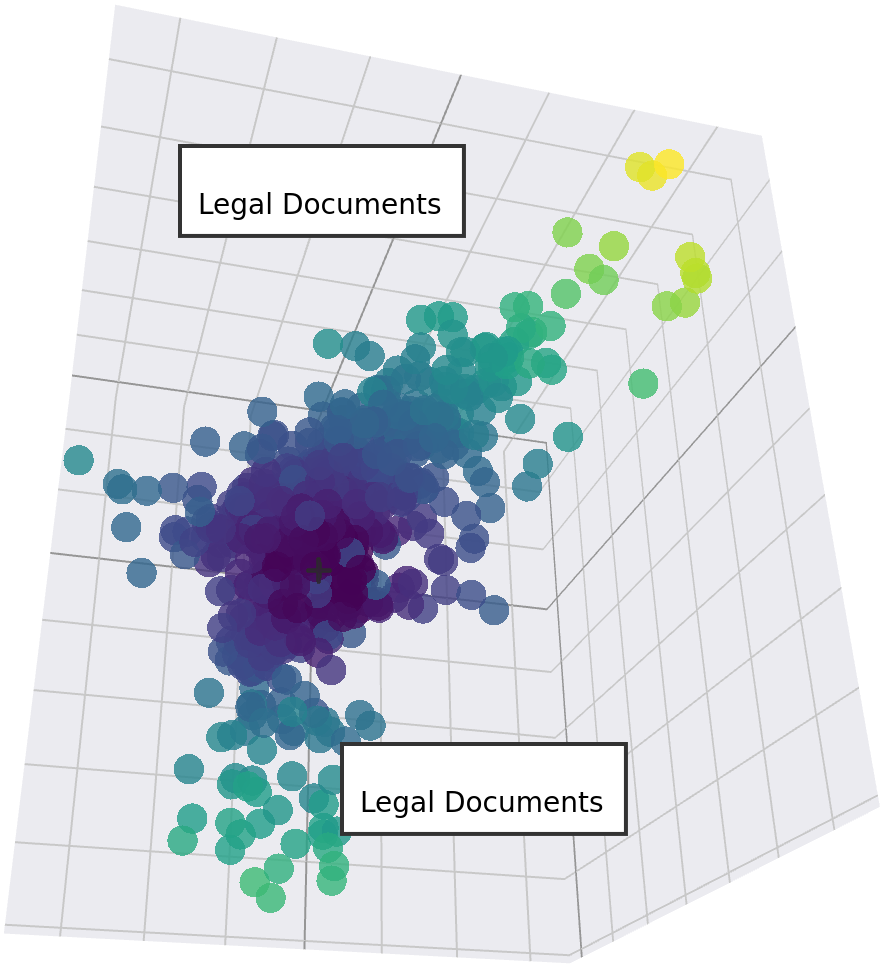
\includegraphics[width=\linewidth,height=4.0cm,keepaspectratio]{paper/camera_ready/gemma_2_9b_l11__continuity__E51__random__cont__0.4423__scatter.png}};
  \node[anchor=north west, inner sep=2pt, overlay] at (img.north west) {\small\textbf{(i)}};
\end{tikzpicture}%
\end{minipage}%
\par\vspace{3pt}%
\begin{minipage}[c][4.0cm][c]{0.3267\linewidth}%
\centering%
\begin{tikzpicture}[baseline=(img.base)]
  \node[inner sep=0pt] (img) {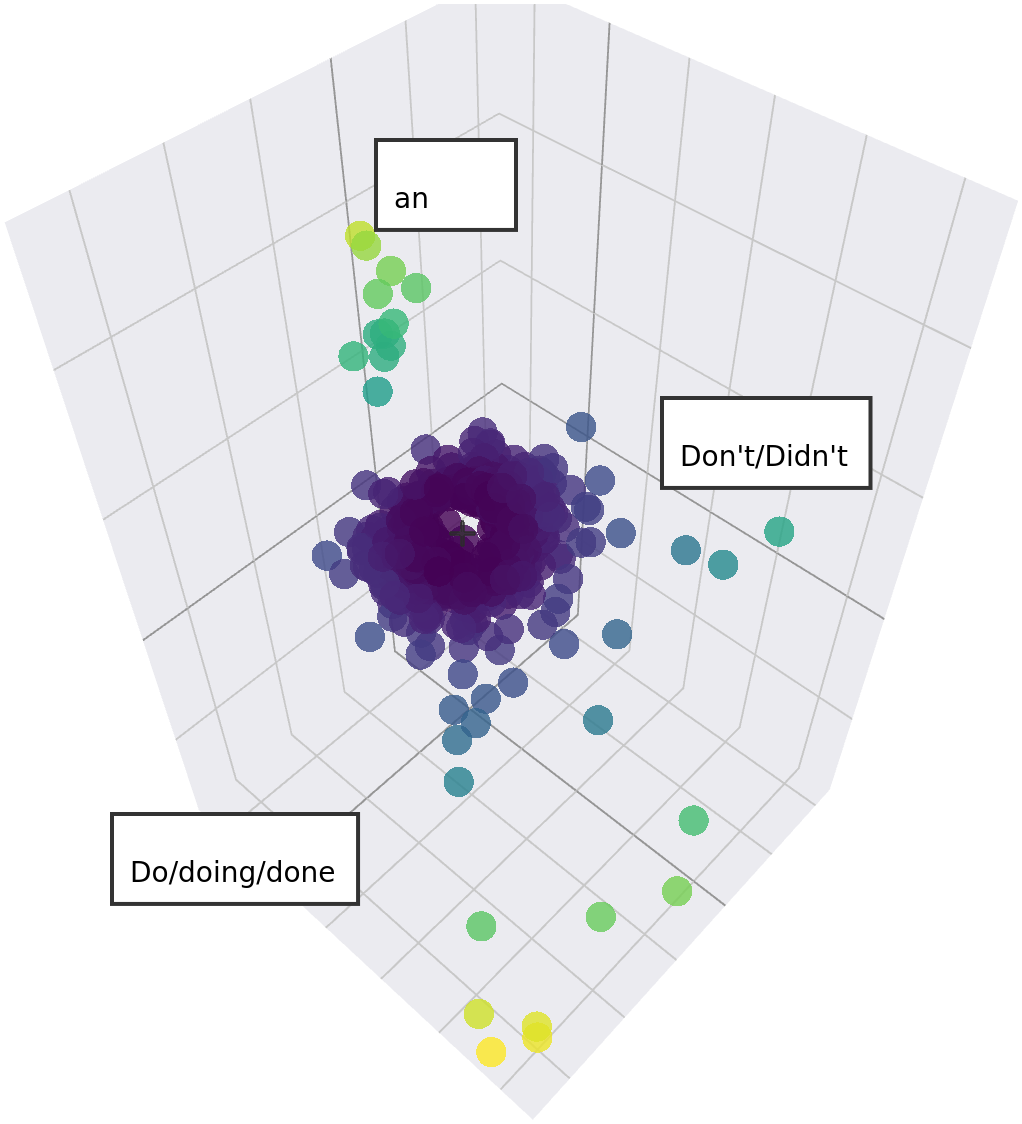
\includegraphics[width=\linewidth,height=4.0cm,keepaspectratio]{paper/camera_ready/gemma_2_9b_l11__continuity__E571__random__cont__0.3260__scatter.png}};
  \node[anchor=north west, inner sep=2pt, overlay] at (img.north west) {\small\textbf{(j)}};
\end{tikzpicture}%
\end{minipage}%
\begin{minipage}[c][4.0cm][c]{0.3267\linewidth}%
\centering%
\vspace{0pt}%
\end{minipage}%
\begin{minipage}[c][4.0cm][c]{0.3267\linewidth}%
\centering%
\vspace{0pt}%
\end{minipage}%
\par\vspace{1pt}%
{\footnotesize\textit{Random Experts (Unlabeled)}}%
\end{minipage}%
}
\caption{Gemma 2 9B, Layer 11. \textbf{Random Experts}: (a) Expert 1326. (b) Expert 1527. (c) Expert 1537. (d) Expert 210. (e) Expert 229. (f) Expert 289. (g) Expert 464. (h) Expert 508. (i) Expert 51. (j) Expert 571. Each plot shows the 3-D bottleneck activations of a single SMIXAE expert; points are individual token activations colored by distance from the origin.}
\label{fig:random_gemma_2_9b_l11}
\end{figure*}
